\documentclass[11pt,a4paper]{article}
\usepackage[utf8]{inputenc}    % Codificación UTF-8 (obligatorio)
\usepackage[T1]{fontenc}       % Soporte para caracteres europeos
\usepackage[spanish]{babel}    % Idioma español (para guiones y nombres)
\usepackage{float}
\usepackage{graphicx}
\usepackage{parskip} 
\usepackage[a4paper, margin=2cm]{geometry}
\usepackage{setspace}
\usepackage{xcolor} 
\usepackage[most]{tcolorbox}
\usepackage{listings}
\usepackage{enumitem} % <-- Para mejor control de listas
\usepackage{inconsolata} % Fuente moderna monoespaciada
\usepackage{fontawesome5} % Para iconos
\usepackage{hyperref}
\usepackage{bookmark} % Handle rerunfilecheck warning
%%% Tabla: 
\usepackage{makecell}       % Para formatear mejor las celdas
\usepackage{multirow}       % Para celdas de múltiples filas
\usepackage{booktabs}       % Mejores líneas horizontales para tablas
\usepackage{colortbl}       % Para colorear celdas
% Definición de colores corporativos (ajústalos según tu preferencia)
\definecolor{headercolor}{RGB}{42, 55, 139}       % Azul oscuro para encabezados
\definecolor{rowcolor1}{RGB}{235, 241, 250}       % Azul muy claro para filas alternas
\definecolor{rowcolor2}{RGB}{255, 255, 255}       % Blanco para filas alternas

% Definición del estilo de cabecera
\newcommand{\headerStyle}[1]{\textcolor{white}{\textbf{#1}}}
% Preambulo para mayor control de las listas de requerimientos funcionales: 
\newcommand{\reqnum}[1]{\textbf{\underline{RF-#1}}}
% Estilo para elementos futuros
\newcommand{\future}[1]{\textit{#1}}


\setstretch{1.2}
% Definir colores modernos
\definecolor{background}{RGB}{250, 250, 252}
\definecolor{comment}{RGB}{92, 122, 158}
\definecolor{keyword}{RGB}{130, 80, 223}
\definecolor{string}{RGB}{64, 160, 112}
\definecolor{number}{RGB}{209, 105, 105}
\definecolor{identifier}{RGB}{36, 41, 46}
\definecolor{frame}{RGB}{232, 234, 237}
\definecolor{caption}{RGB}{42, 44, 57}

% Estilo para JSON
\lstdefinelanguage{json}{
    basicstyle=\fontfamily{zi4}\selectfont\footnotesize,
    commentstyle=\color{comment}\itshape,
    keywordstyle=\color{keyword}\bfseries,
    numberstyle=\tiny\color{number},
    stringstyle=\color{string},
    breakatwhitespace=false,
    breaklines=true,
    keepspaces=true,
    numbers=left,
    numbersep=10pt,
    showspaces=false,
    showstringspaces=false,
    showtabs=false,
    tabsize=2,
    morestring=[b]",
    morekeywords={true,false,null}
}

% Estilo para HTTP
\lstdefinelanguage{HTTP}{
    morekeywords={GET,POST,PUT,DELETE,HEAD,OPTIONS,PATCH},
    sensitive=false,
    morecomment=[l]{//},
    morecomment=[s]{/*}{*/},
    morestring=[b]",
    basicstyle=\fontfamily{zi4}\selectfont\footnotesize\color{identifier},
    keywordstyle=\color{keyword}\bfseries,
}

% Estilo para JavaScript
\lstdefinelanguage{JavaScript}{
    keywords={typeof, new, true, false, catch, function, return, null, catch, switch, var, if, in, while, do, else, case, break},
    keywordstyle=\color{keyword}\bfseries,
    ndkeywords={class, export, boolean, throw, implements, import, this},
    ndkeywordstyle=\color{number}\bfseries,
    identifierstyle=\color{identifier},
    sensitive=false,
    comment=[l]{//},
    morecomment=[s]{/*}{*/},
    morestring=[b]',
    morestring=[b]",
    basicstyle=\fontfamily{zi4}\selectfont\footnotesize\color{identifier},
}

% Definir entorno personalizado para los bloques de código
\newtcolorbox{codebox}[2][]{
    colback=background,
    colframe=frame,
    boxrule=1pt,
    title=#2,
    before skip=10pt,
    after skip=10pt,
    #1
}

% Configuración global para listings
\lstset{
    basicstyle=\fontfamily{zi4}\selectfont\footnotesize\color{identifier},
    commentstyle=\color{comment},
    breaklines=true,
    backgroundcolor=\color{background},
    frame=none,
    framesep=5pt,
    xleftmargin=15pt,
    numbers=left,
    numberstyle=\tiny\color{comment},
    stepnumber=1,
    numbersep=10pt,
    captionpos=t,
}


\title{Documento de arquitectura y desarrollo del sistema SID}
\author{Henry Ricaurte Mora}
\date{Abril de 2025}

\begin{document}

\maketitle

\tableofcontents

\newpage

\section{Introducción}

En esta sección se brinda una visión introductoria de los conceptos relacionados con la descripción del sistema del SID.
Es importante establecer una estructura clara de los componentes que lo conforman.

\begin{figure}[htbp]
	\centering
	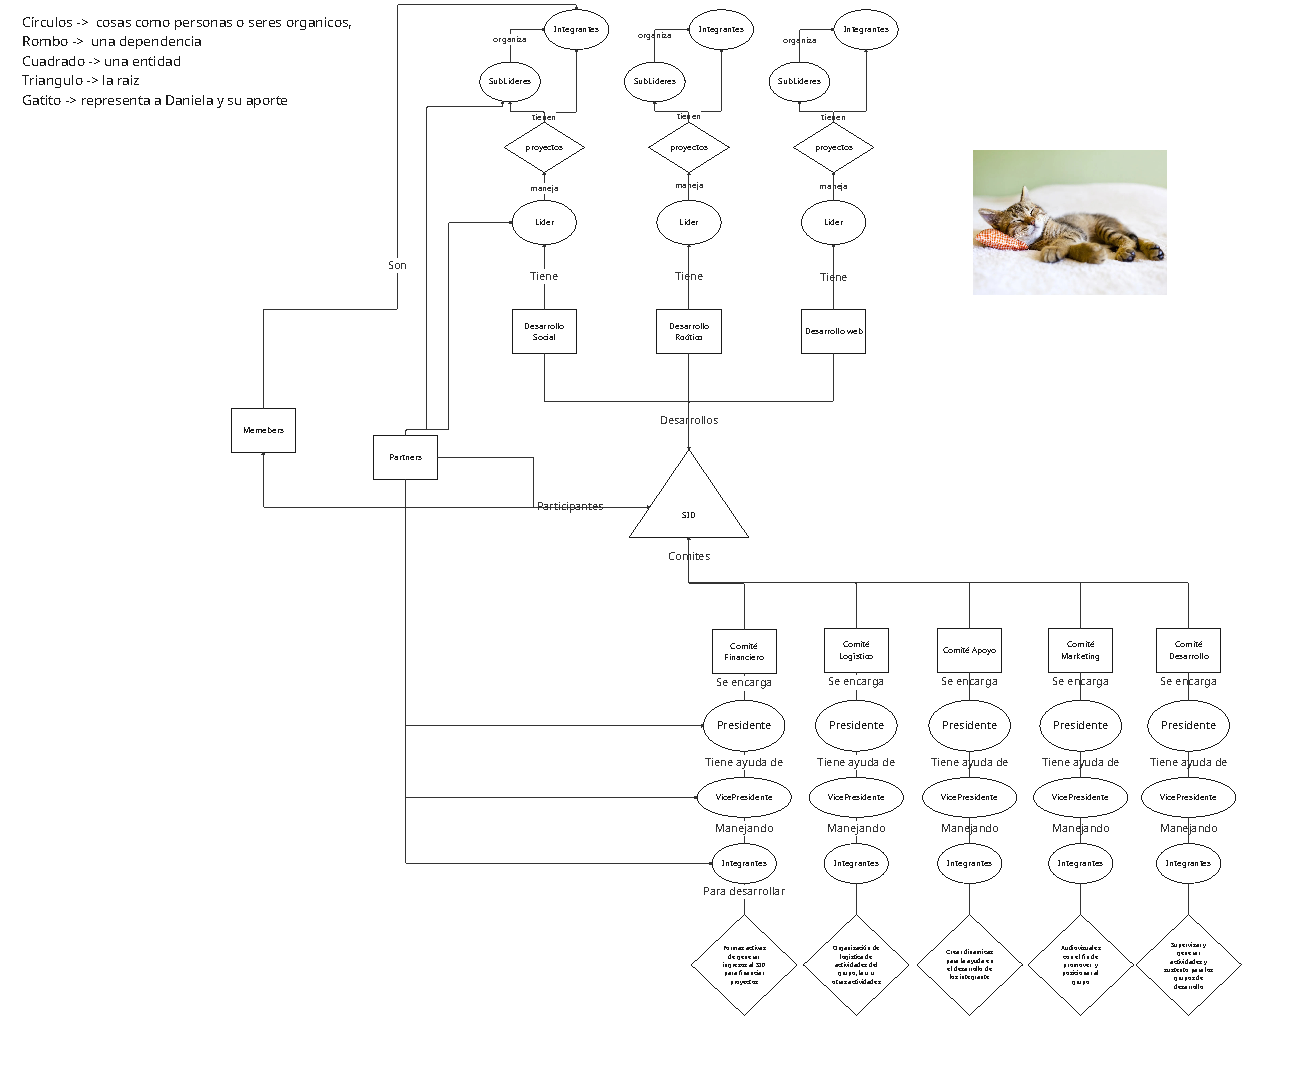
\includegraphics[width=0.8\textwidth]{src/SID_org.pdf}
	\caption{Diagrama de organización del SID}
\end{figure}

El SID está conformado por tres ramas principales:

\begin{itemize}
	\item \textbf{Desarrollos:} Social, Robótico y Web.
	\item \textbf{Comités:} Financiera, Logística, Apoyo, Marketing y Desarrollo.
	\item \textbf{Participantes:} \textit{Partners} y \textit{Members}.
\end{itemize}

\subsection{Comités}

Los comités son responsables del funcionamiento del SID. Cada uno tiene un presidente y un vicepresidente,
quienes lideran al equipo para desarrollar estrategias como:

\begin{itemize}
	\item Generar ingresos para financiar proyectos.
	\item Organizar la logística de las actividades.
	\item Establecer dinámicas de formación para los integrantes.
	\item Crear contenido audiovisual para promoción.
	\item Supervisar y respaldar a los grupos de desarrollo.
\end{itemize}

\subsection{Desarrollos}

Cada desarrollo (Social, Robótico y Web) cuenta con un líder, sublíderes y un equipo.
El líder coordina el proyecto general, los sublíderes gestionan apartados específicos y los integrantes trabajan bajo su guía.

Por ejemplo, este documento forma parte de un proyecto en el desarrollo Web.

\paragraph{}
Los \textit{Partners} incluyen a presidentes, vicepresidentes, líderes y sublíderes. Los \textit{Members} son
integrantes que participan activamente en cada uno de los apartados de desarrollo.

\section{Descripción General del Sistema}
Se desarrollará una plataforma integral para la gestión y difusión de información del grupo SID. Esta incluirá herramientas para la presentación institucional, la oferta de cursos de formación y la divulgación de conocimiento especializado.

\subsection{Componentes Principales}
\begin{itemize}
	\item \textbf{Portal Web Principal: } Será el sitio informativo del grupo,
	      donde se mostrará quiénes somos y cuáles son nuestras áreas de trabajo. Este portal incluirá secciones dedicadas a los distintos
	      desarrollos del grupo, cada una con su propia página que detallará a sus integrantes, proyectos y líderes. Asimismo, se presentarán los
	      comités con una estructura similar.
	      También se incluirá información general sobre el SID, sus actividades, proyectos, equipos, colaboraciones, cursos, noticias e integrantes,
	      además de un formulario de inscripción para nuevos miembros o interesados.

	\item \textbf{Panel Administrativo: } Permitirá la gestión del contenido visible en el portal principal, así como la administración de los datos de los usuarios provenientes de los formularios de inscripción.

	\item \textbf{Sistema de Gestión Académica: } Este componente permitirá la inscripción y administración de los cursos ofrecidos. Incluirá funcionalidades específicas para tres tipos de usuarios: administrador, profesor y estudiante/usuario. También facilitará la asignación y gestión de profesores por curso.

	\item \textbf{SID Academy: } Proyecto futuro que se plantea como una plataforma educativa de cursos breves, similar a QtAcademy, con el objetivo de fortalecer el aprendizaje especializado dentro de la comunidad.
\end{itemize}

\section{Requerimientos del Sistema}
\subsection{Requerimientos Funcionales: }
\subsubsection{Portal Web Principal}
\begin{enumerate}[leftmargin=*,labelwidth=2.5cm,align=left]
	\item[\reqnum{001}] El sistema debe mostrar información institucional del grupo SID.
	\item[\reqnum{002}] El sistema debe presentar secciones para cada desarrollo del grupo (Web, Robótica, Social) con sus integrantes, proyectos y líderes.
	\item[\reqnum{003}] El sistema debe mostrar información sobre los comités existentes.
	\item[\reqnum{004}] El sistema debe listar actividades realizadas por el grupo.
	\item[\reqnum{005}] El sistema debe mostrar proyectos desarrollados por el grupo.
	\item[\reqnum{006}] El sistema debe exponer los cursos ofrecidos por el grupo.
	\item[\reqnum{007}] El sistema debe presentar los equipos de trabajo.
	\item[\reqnum{008}] El sistema debe publicar noticias relacionadas con el grupo.
	\item[\reqnum{009}] El sistema debe mostrar información sobre fundaciones y colaboraciones.
	\item[\reqnum{010}] El sistema debe incluir un formulario de inscripción para nuevos miembros.
\end{enumerate}

\subsubsection{Panel Administrativo (Dashboard)}
\begin{enumerate}[leftmargin=*,labelwidth=2.5cm,align=left,start=11]
	\item[\reqnum{011}] El sistema debe permitir a los administradores gestionar el contenido del portal web.
	\item[\reqnum{012}] El sistema debe proporcionar funcionalidades para administrar los datos de usuarios.
	\item[\reqnum{013}] El sistema debe permitir la gestión de actividades (crear, modificar, eliminar).
	\item[\reqnum{014}] El sistema debe permitir la gestión de proyectos (crear, modificar, eliminar).
	\item[\reqnum{015}] El sistema debe permitir la gestión de cursos (crear, modificar, eliminar).
	\item[\reqnum{016}] El sistema debe permitir la gestión de equipos (crear, modificar, eliminar).
	\item[\reqnum{017}] El sistema debe permitir la gestión de noticias (crear, modificar, eliminar).
	\item[\reqnum{018}] El sistema debe permitir la gestión de fundaciones (crear, modificar, eliminar).
	\item[\reqnum{019}] El sistema debe implementar control de acceso basado en roles.
	\item[\reqnum{020}] El sistema debe permitir la administración de permisos por rol.
\end{enumerate}

\subsubsection{API de Servicios}
\begin{enumerate}[leftmargin=*,labelwidth=2.5cm,align=left,start=21]
	\item[\reqnum{021}] El sistema debe proporcionar endpoints RESTful para listar contenido (actividades, proyectos, etc.).
	\item[\reqnum{022}] El sistema debe implementar paginación en todos los endpoints que devuelven listas.
	\item[\reqnum{023}] El sistema debe manejar formatos estándar para solicitudes y respuestas (JSON).
	\item[\reqnum{024}] El sistema debe implementar autenticación mediante tokens JWT.
	\item[\reqnum{025}] El sistema debe proporcionar endpoints para la gestión de contenidos protegidos por autenticación.
\end{enumerate}

\subsection{Requerimientos No Funcionales}

\subsubsection{Seguridad}
\begin{enumerate}[leftmargin=*,labelwidth=2.5cm,align=left]
	\item[\reqnum{026}] El sistema debe implementar autenticación OAuth 2.0 con proveedores de identidad externos (Microsoft Entra ID/Azure AD / Google).
	\item[\reqnum{027}] El sistema debe validar y procesar tokens JWT emitidos por el proveedor de identidad.
	\item[\reqnum{028}] El sistema debe implementar control de acceso basado en roles mediante la base de datos
	\item[\reqnum{029}] El sistema debe proteger los endpoints administrativos con autorización basada en roles
	\item[\reqnum{030}] El sistema debe usar HTTPS para todas las comunicaciones (TLS 1.2+). | Toca entender que es a profundidad
	\item[\reqnum{031}] El sistema debe implementar protección contra ataques comunes (CSRF, XSS, SQL Injection).
\end{enumerate}

\subsubsection{Rendimiento}
\begin{enumerate}[leftmargin=*,labelwidth=2.5cm,align=left,start=32]
	\item[\reqnum{032}] El sistema debe responder a las solicitudes API en menos de 1 segundo bajo carga normal.
	\item[\reqnum{033}] El sistema debe soportar al menos 100 usuarios concurrentes.
	\item[\reqnum{034}] Las consultas a la base de datos deben optimizarse para minimizar el tiempo de respuesta.
\end{enumerate}

\subsubsection{Escalabilidad}
\begin{enumerate}[leftmargin=*,labelwidth=2.5cm,align=left,start=35]
	\item[\reqnum{035}] La arquitectura debe permitir escalar componentes individuales según demanda.
	\item[\reqnum{036}] El sistema debe ser compatible con despliegue en contenedores (Docker/Kubernetes).
\end{enumerate}

\subsubsection{Mantenibilidad}
\begin{enumerate}[leftmargin=*,labelwidth=2.5cm,align=left,start=37]
	\item[\reqnum{037}] El código debe seguir los principios SOLID y patrones de diseño apropiados.
	\item[\reqnum{038}] El sistema debe implementar logging estructurado (JSON) para diagnóstico.
	\item[\reqnum{039}] El código debe incluir documentación JavaDoc y OpenAPI para las APIs.
\end{enumerate}

\subsubsection{Compatibilidad}
\begin{enumerate}[leftmargin=*,labelwidth=2.5cm,align=left,start=40]
	\item[\reqnum{040}] Las APIs deben seguir el estándar RESTful nivel 2 de Richardson.
	\item[\reqnum{041}] El sistema debe proporcionar documentación interactiva mediante Swagger UI.
\end{enumerate}

\subsubsection{Interoperabilidad}
\begin{enumerate}[leftmargin=*,labelwidth=2.5cm,align=left,start=44]
	\item[\reqnum{044}] El sistema debe exponer APIs con versionado semántico (v1, v2). | Acordar si mandarlo en header o en la api. (obligatorio tag github)
	\item[\reqnum{045}] Las integraciones deben usar protocolos estándar (OAuth 2.0, OpenID Connect).
\end{enumerate}



\section{Especificación Modulos:}

\begin{figure}[H]
	\centering
	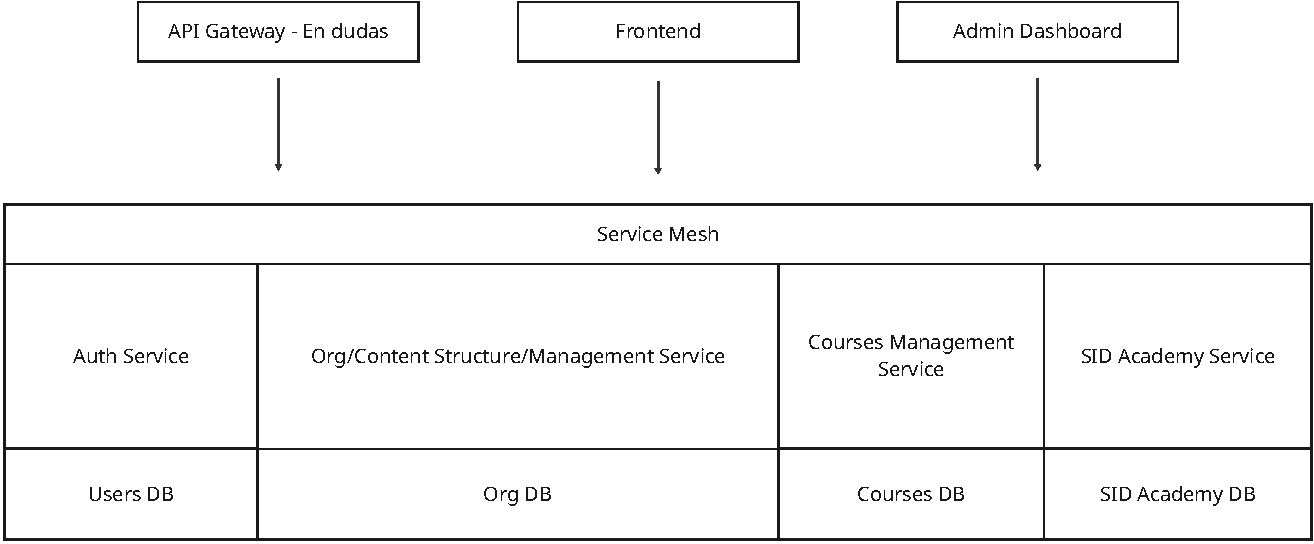
\includegraphics[width=0.5\textwidth]{src/SID_microservices.pdf}
	\caption{Diagrama de modulos del proyecto}
\end{figure}

% \subsection{Servicio de Autenticación y Usuarios}
% \begin{itemize}
% 	\item Gestión completa del ciclo de vida de usuarios
% 	\item Autenticación y autorización
% 	\item Gestión de tokens y sesiones
% \end{itemize}

% \subsection{Servicio del portal web y dashboard}
% \begin{itemize}
% 	\item Visualización de desarrollos (Web, Robótica, etc.)
% 	\item Visualización de comités (Financiero, Social, etc.)
% 	\item Visualización de noticias y actualizaciones
% 	\item Visualización de información sobre fundaciones y trabajos realizados
% 	\item Visualización de integrantes y Formulario

% 	\item Administración y gestión de desarrollos (Web, Robótica, etc.)
% 	\item Administración y gestión de comités (Financiero, Social, etc.)
% 	\item Administración y gestión de noticias y actualizaciones
% 	\item Administración y gestión de información sobre fundaciones y trabajos realizados
% 	\item Administración y gestión de integrantes
% 	\item Administracion de integrantes mediante Formulario.
% \end{itemize}

% \subsection{Servicio de gestión de cursos}
% \begin{itemize}
% 	\item Catálogo e inscripción a cursos
% 	\item Gestión de profesores y alumnos
% 	\item Seguimiento y evaluación
% \end{itemize}

% \subsection{Servicio SIDAcademy (futuro)}
% \begin{itemize}
% 	\item Gestión de contenidos educativos cortos
% 	\item Sistema de aprobación y curación
% 	\item Análisis de métricas de consumo
% \end{itemize}


\begin{table}[H]
	\centering
	\renewcommand{\arraystretch}{1.5}
	\begin{tabular}{>{\raggedright\arraybackslash}p{2.8cm} >{\raggedright\arraybackslash}p{5.0cm} >{\raggedright\arraybackslash}p{3.0cm} >{\raggedright\arraybackslash}p{3.0cm}}
		\toprule
		\rowcolor{headercolor}
		\headerStyle{M{\'o}dulo}                   & \headerStyle{Función principal} & \headerStyle{Métodos API} & \headerStyle{Seguridad} \\
		\midrule
		\rowcolor{rowcolor1}
		\textbf{AuthService}                       &
		Autenticación y autorización\newline
		Gestión de usuarios y roles\newline
		Administración de tokens y sesiones        &
		\begin{itemize}[nosep,leftmargin=*]
			\item POST
			\item GET
			\item PUT
		\end{itemize}        &
		JWT\newline
		(Solo login es público)                                                                                                            \\
		\midrule
		\rowcolor{rowcolor2}
		\textbf{PortalService y Dashboard control} &
		Visualización pública del SID\newline
		(desarrollos, comités, noticias)\newline
		Administración de desarrollos\newline
		Gestión de comités y fundaciones           &
		\begin{itemize}[nosep,leftmargin=*]
			\item GET
			\item POST
			\item PUT
			\item PATCH
			\item DELETE
		\end{itemize}        &
		Mixto:\newline
		• Público (lectura)\newline
		• JWT + roles (escritura)                                                                                                          \\
		\midrule
		\rowcolor{rowcolor1}
		\textbf{CoursesService}                    &
		Gestión de cursos e inscripciones\newline
		Administración de profesores/alumnos\newline
		Seguimiento y evaluación académica         &
		\begin{itemize}[nosep,leftmargin=*]
			\item GET
			\item POST
			\item PUT
		\end{itemize}        &
		JWT + roles\newline
		(basado en perfiles académicos)                                                                                                    \\
		\midrule
		\rowcolor{rowcolor2}
		\textbf{\future{SIDAcademy}}\newline
		\textit{(futuro)}                          &
		Contenidos educativos cortos\newline
		Curación de material didáctico\newline
		Análisis de métricas de aprendizaje        &
		\begin{itemize}[nosep,leftmargin=*]
			\item GET
			\item POST
			\item PUT
		\end{itemize}        &
		JWT + roles\newline
		(según nivel de acceso)                                                                                                            \\
		\bottomrule
	\end{tabular}
	\caption{Arquitectura de modulos propuesta para el sistema SID}
\end{table}
\section{Arquitectura de Base de Datos: }
Como base de datos se elige una NewSQL como Neon la cual opera con postgresql, elegido por comidad de diseño y ademas brinda lo necesario para el proyecto.
La base de datos generada es:
\begin{figure}[H]
	\centering
	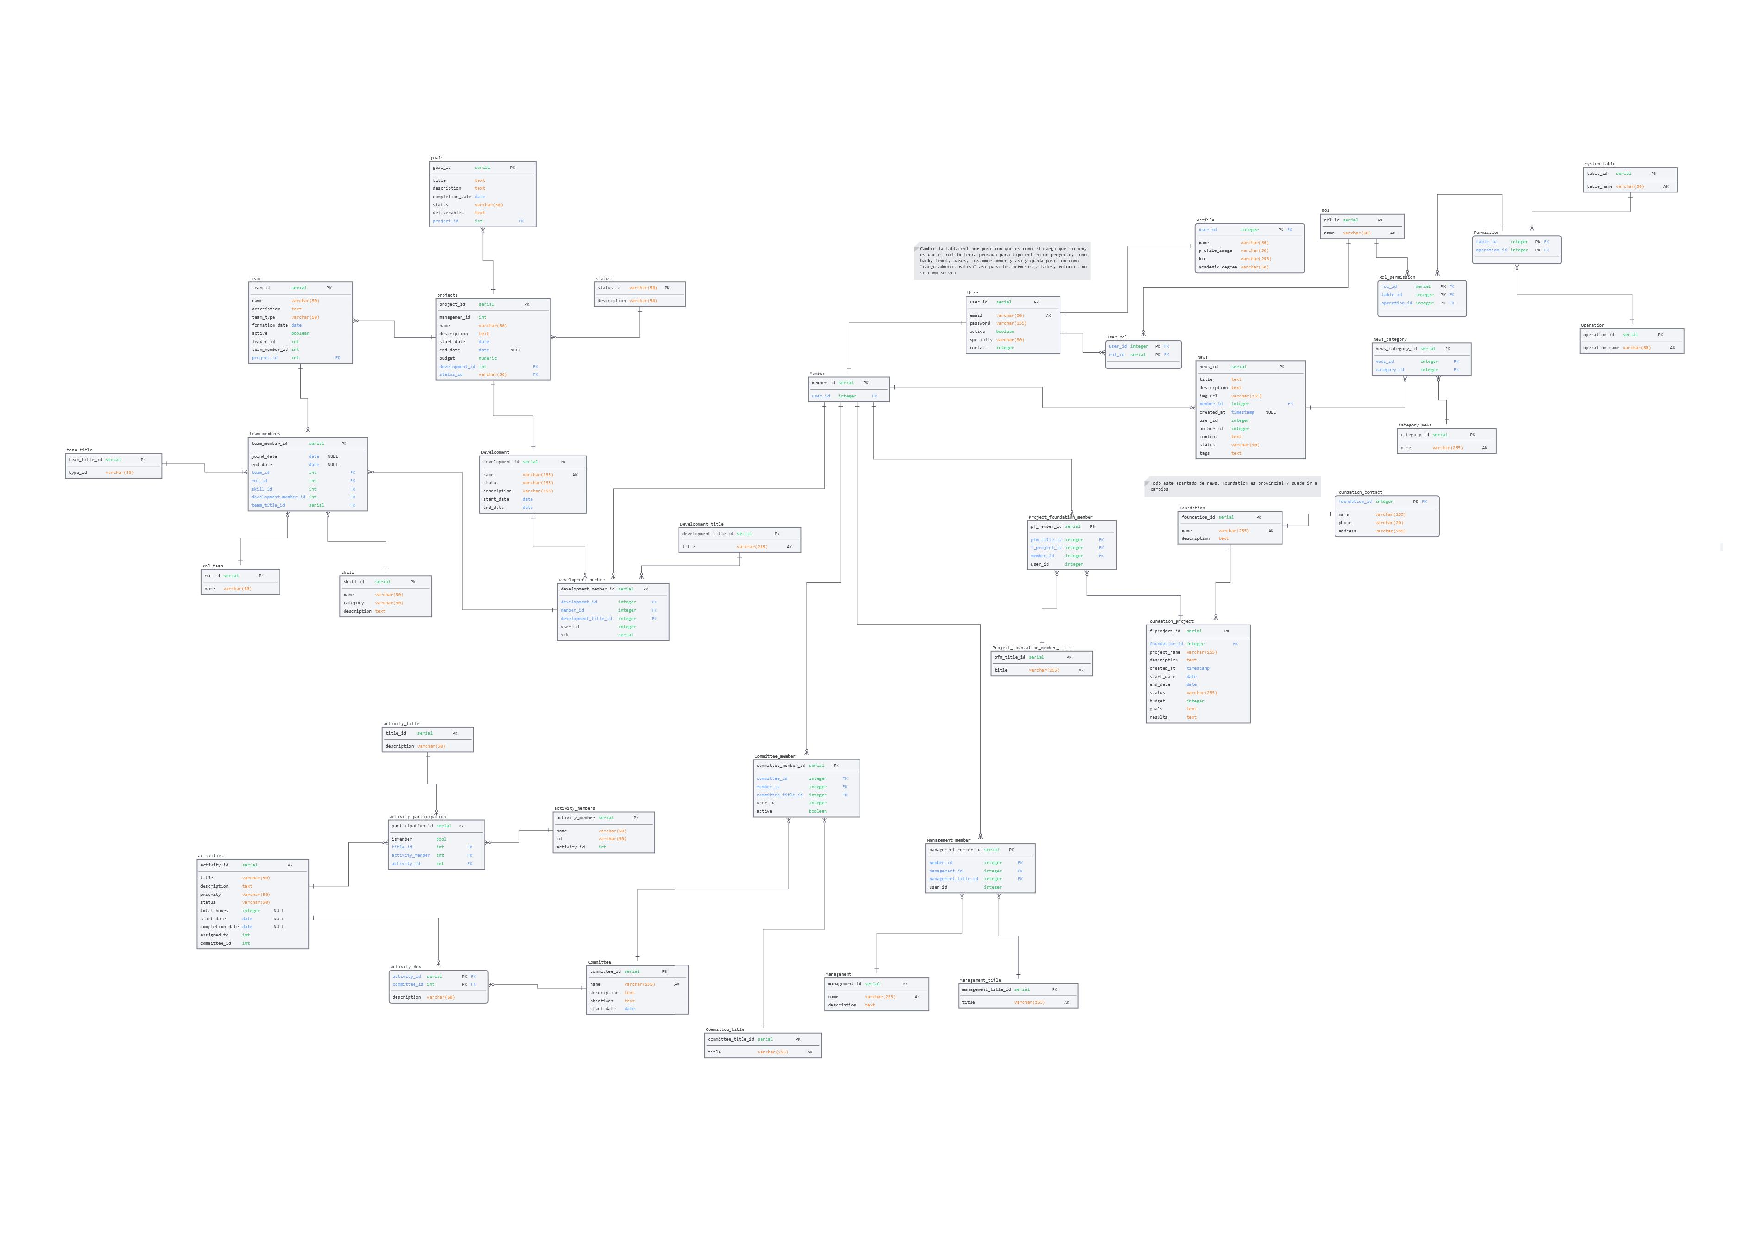
\includegraphics[width=0.5\textwidth]{src/ModeloTerminado.pdf}
	\caption{Diagrama de base de datos relacional}
\end{figure}

\section{Arquitectura Portal Content Service}
Este servicio de portal de contenido que se generará es la dicha ``Página del SID'', desde el lado del backend tenemos que suplir información relevante,
esta información está dividida en:
\begin{itemize}
	\item Actividades
	\item Proyectos
	\item Cursos
	\item Equipos
	\item Noticias
	\item Aliados | Fundaciones
\end{itemize}

\subsection{Vision General}
El diseño del sistema sigue un patrón de arquitectura estándar de múltiples capas comúnmente utilizado en aplicaciones de SpringBoot.
El sistema está diseñado para mantener el desacoplamiento de funciones para garantizar la mantenibilidad, la comprobabilidad (Testing) y la
escalabilidad
\begin{figure}[H]
	\centering
	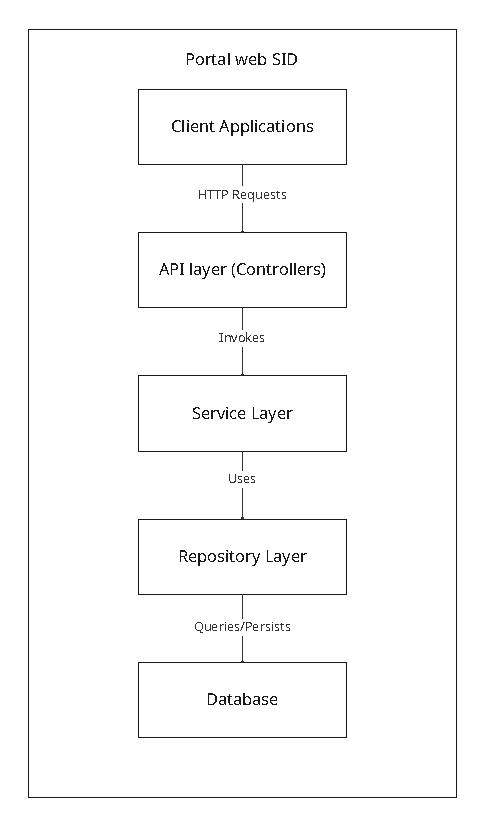
\includegraphics[width=0.4\textwidth]{src/SID_PortalWEB_D1.pdf}
	\caption{Diagrama de la arquitectura por capas}
\end{figure}

\begin{table}[h!]
	\centering
	\begin{tabular}{|l|p{4cm}|p{7cm}|}
		\hline
		\textbf{Capa}       & \textbf{Descripción}                              & \textbf{Responsabilidades principales}                                       \\
		\hline
		Capa API            & Punto de entrada para las solicitudes del cliente & Manejo de solicitudes, formateo de respuestas, validación de entradas        \\
		\hline
		Capa de Servicio    & Contiene la lógica de la aplicación               & Orquesta operaciones, maneja transacciones y logica de la aplicación         \\
		\hline
		Capa de Repositorio & Gestiona el acceso a los datos                    & Proporciona una abstracción sobre el almacenamiento, maneja operaciones CRUD \\
		\hline
		Capa de Dominio     & Contiene las entidades del dominio                & Encapsula los datos y la lógica del negocio                                  \\
		\hline
	\end{tabular}
	\caption{Responsabilidades por capa del sistema}
\end{table}

\subsection{Capa API (Controladores)}

La capa API es responsable de manejar las solicitudes HTTP entrantes, validar los datos de entrada y devolver respuestas apropiadas.
Esta capa está compuesta por clases controladoras que definen los endpoints REST expuestos por la aplicación.

Los controladores siguen la convención REST tanto para el nombramiento de endpoints como para el uso de métodos HTTP:

\begin{itemize}
	\item \textbf{GET} para obtener recursos
	\item \textbf{POST} para crear recursos
	\item \textbf{PUT} para actualizar recursos completamente
	\item \textbf{PATCH} para actualizar parcialmente recursos
	\item \textbf{DELETE} para eliminar recursos
\end{itemize}

\subsection{Capa de Servicio}

La capa de servicio implementa la lógica central de la aplicación.
Se ubica entre los controladores y los repositorios, orquestando operaciones entre múltiples entidades del dominio y aplicando las reglas de negocio.

\subsection{Capa de Repositorio}

La capa de repositorio proporciona una abstracción sobre el mecanismo de acceso a datos.
Utiliza Spring Data JPA para simplificar las operaciones con la base de datos y reducir el código repetitivo.
También en los casos necesarios utiliza el patrón repositorio para hacer llamados directos a la base de datos de ser necesario

\subsection{Capa de Dominio}

La capa de dominio contiene las clases de entidad que representan el dominio del negocio.
Estas clases son aquellas que sirven para encapsular la logica del negocio, y se pasa a service para ser manejada.

\subsection{Capa de Entidad}
La capa de entidad proporciona aquellas clases que representan la abstracción más cercana a la base de datos.
Son quienes se usaran mediante los JPA para hacer llamados directos a la base de datos y tambien usada en los repositorios manuales

\subsection{Flujo de peticiones}
\begin{figure}[H]
	\centering
	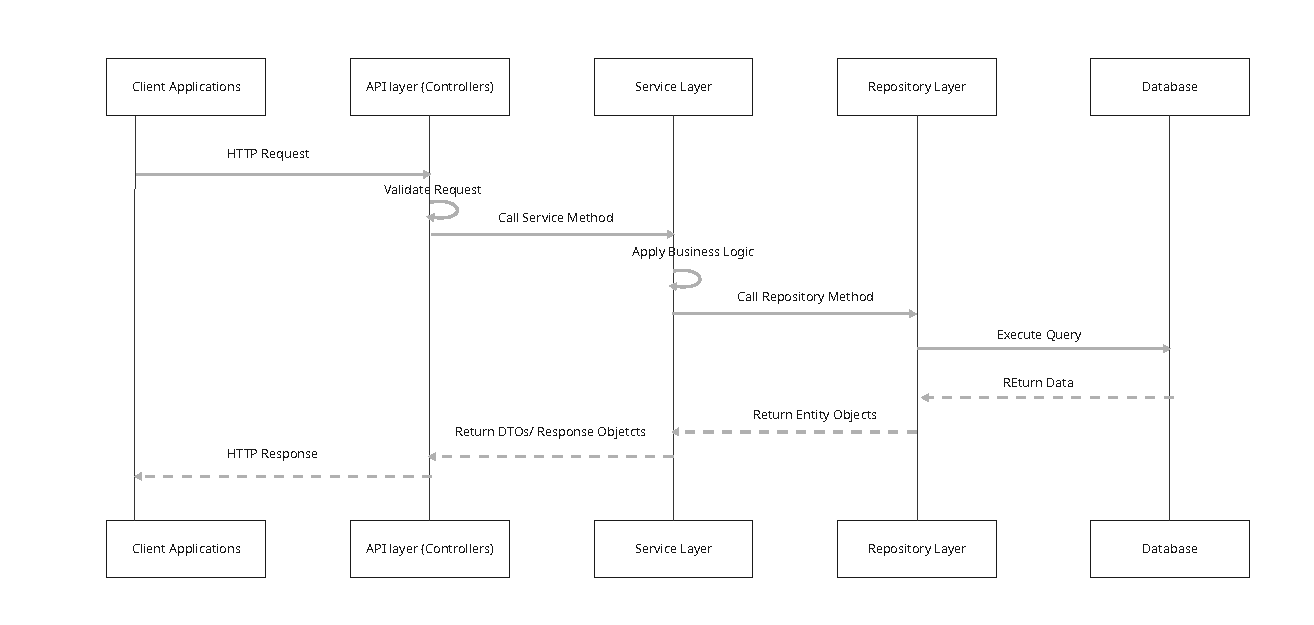
\includegraphics[width=0.5\textwidth]{src/SID_request-flow.pdf}
	\caption{Diagrama de el flujo de las petciones por capas}
\end{figure}

\subsection{Endpoints REST}
Con base en los elementos anteriores, definimos los siguientes endpoints REST con paginación de Spring Boot:

%%%%%%%%%%%%%%%%%%%%%%%%%%%%%   ACTIVIDADES %%%%%%%%%%%%%%%%%%%%

\subsubsection{Actividades}

\paragraph{GET Todos (Paginado)}

\begin{center}
	\begin{minipage}{\textwidth}
		\begin{codebox}{GET Actividades (paginado)}
			\begin{lstlisting}[language=HTTP]
GET /api/activities?page=0&size=10&sort=startDate,desc
\end{lstlisting}
		\end{codebox}
	\end{minipage}
\end{center}

\begin{center}
	\begin{minipage}{\textwidth}
		\begin{codebox}{Estructura de respuesta}
			\begin{lstlisting}[language=json]
{
    "content": [
        {
            "id": integer,                   // ID unico de la actividad
            "title": string,                 // Titulo de la actividad
            "description": string,           // Descripcion de la actividad
            "priority": string(enum),        // Prioridad: "ALTA", "MEDIA", "BAJA"
            "status": string(enum),          // Estado: "ACTIVA", "ESPERA", "COMPLETADA", "CANCELADA"
            "total_hours": integer,          // Total de horas estimadas
            "start_date": string(ISO-8601),  // Fecha de inicio
            "completation_date": string(ISO-8601), // Fecha estimada de finalizacion
            "manager": string,               // Nombre del gestor de la actividad
            "created_at": string(ISO-8601)   // Fecha de creacion
        }
        // ... mas elementos
    ],
    "pageable": {
        "sort": object,       // Informacion de ordenamiento
        "pageSize": integer,  // Tamanioo de pagina solicitado
        "pageNumber": integer // Numero de pagina actual
        // ... mas metadatos de paginacion
    },
    "totalElements": integer, // Total de resultados
    "totalPages": integer,    // Total de paginas disponibles
    "first": boolean,         // Si es la primera pagina
    "last": boolean,          // Si es la ultima pagina
    "size": integer           // Tamanio de la pagina actual
}
\end{lstlisting}
		\end{codebox}
	\end{minipage}
\end{center}

\paragraph{GET Individual}

\begin{center}
	\begin{minipage}{\textwidth}
		\begin{codebox}{GET /api/activities/{id} - Obtener actividad específica}
			\begin{lstlisting}[language=HTTP]
GET /api/activities/{id}
\end{lstlisting}
		\end{codebox}
	\end{minipage}
\end{center}

\begin{center}
	\begin{minipage}{\textwidth}
		\begin{codebox}{Estructura de respuesta}
			\begin{lstlisting}[language=json]
{
    "id": integer,                   // ID unico
    "title": string,                 // Titulo de la actividad
    "description": string,           // Descripcion detallada
    "priority": string(enum),        // Prioridad: "ALTA", "MEDIA", "BAJA"
    "status": string(enum),          // Estado: "ACTIVA", "ESPERA", "COMPLETADA", "CANCELADA"
    "total_hours": integer,          // Total de horas estimadas
    "start_date": string(ISO-8601),  // Fecha de inicio
    "completation_date": string(ISO-8601), // Fecha estimada de finalizacion
    "manager": string,               // Nombre del gestor
    "members": [                     // Miembros asignados
        {
            "name": string,          // Nombre del miembro
            "identify": string,      // Identificador unico
            "isMember": boolean      // Si es miembro del SID
        },
        // ... mas miembros
    ],
    "committees": [                  // Comites asociados
        {
            "name": string,          // Nombre del comite
            "leader": string,        // Lider del comite
            "description": string    // Descripcion de funcion
        },
        // ... mas comites
    ]
}
\end{lstlisting}
		\end{codebox}
	\end{minipage}
\end{center}

\paragraph{POST Creación}
\begin{center}
	\begin{minipage}{\textwidth}
		\begin{codebox}{POST /api/activities - Crear nueva actividad}
			\begin{lstlisting}[language=HTTP]
POST /api/activities
Content-Type: application/json
Authorization: Bearer <token>

{
    "title": string,                 // Requerido: Titulo de la actividad
    "description": string,           // Requerido: Descripcion
    "priority": string(enum),        // Requerido: "ALTA", "MEDIA", "BAJA"
    "status": string(enum),          // Requerido: "ACTIVA", "ESPERA", "COMPLETADA", "CANCELADA"
    "total_hours": integer,          // Requerido: Horas estimadas
    "start_date": string(ISO-8601),  // Requerido: Fecha de inicio
    "completation_date": string(ISO-8601), // Requerido: Fecha estimada de finalizacion
    "manager": string,               // Requerido: Nombre del gestor
    "members": [                     // Opcional: Miembros asignados
        {
            "name": string,          // Nombre del miembro
            "identify": string,      // Identificador unico
            "isMember": boolean      // Si es miembro del SID
        },
        // ... mas miembros
    ],
    "committees": [                  // Opcional: Comites asociados
        {
            "committee_id": integer, // ID del comite existente
            "description": string    // Descripcion de funcion
        },
        // ... mas comites
    ]
}
\end{lstlisting}
		\end{codebox}
	\end{minipage}
\end{center}

\begin{center}
	\begin{minipage}{\textwidth}
		\begin{codebox}{Estructura de respuesta}
			\begin{lstlisting}[language=json]
{
    "code": integer,    // Codigo de respuesta
    "message": string   // Mensaje de exito
}
\end{lstlisting}
		\end{codebox}
	\end{minipage}
\end{center}

\paragraph{PUT (Reemplazo completo)}
\begin{center}
	\begin{minipage}{\textwidth}
		\begin{codebox}{PUT /api/activities/{id} - Actualizar actividad completa}
			\begin{lstlisting}[language=HTTP]
PUT /api/activities/{id}
Content-Type: application/json
Authorization: Bearer <token>

{
    "title": string,                 // Requerido: Nuevo titulo
    "description": string,           // Requerido: Nueva descripcion
    "priority": string(enum),        // Requerido: Nueva prioridad
    "status": string(enum),          // Requerido: Nuevo estado
    "total_hours": integer,          // Requerido: Nuevas horas estimadas
    "start_date": string(ISO-8601),  // Requerido: Nueva fecha de inicio
    "completation_date": string(ISO-8601), // Requerido: Nueva fecha de finalizacion
    "manager": string,               // Requerido: Nuevo gestor
    "members": [                     // Requerido: Nuevos miembros
        {
            "name": string,
            "identify": string,
            "isMember": boolean
        }
        // ... todos los miembros
    ],
    "committees": [                  // Requerido: Nuevos comites
        {
            "committee_id": integer,
            "description": string
        }
        // ... todos los comites
    ]
}
\end{lstlisting}
		\end{codebox}
	\end{minipage}
\end{center}

\begin{center}
	\begin{minipage}{\textwidth}
		\begin{codebox}{Estructura de respuesta}
			\begin{lstlisting}[language=json]
{
    "code": integer,    // Codigo de respuesta
    "message": string   // Mensaje de exito
}
\end{lstlisting}
		\end{codebox}
	\end{minipage}
\end{center}

\paragraph{PATCH (Actualización parcial)}
\begin{center}
	\begin{minipage}{\textwidth}
		\begin{codebox}{PATCH /api/activities/{id} - Actualizar campos específicos}
			\begin{lstlisting}[language=HTTP]
PATCH /api/activities/{id}
Content-Type: application/json-patch+json
Authorization: Bearer <token>

[
    { 
      "op": string(enum), 
      "path": string, 
      "value": any 
    }, // Operacion JSON Patch
    // Operaciones permitidas: "replace", "add", "remove"
    // Ejemplo: { "op": "replace", "path": "/status", "value": "COMPLETADA" }
]
\end{lstlisting}
		\end{codebox}
	\end{minipage}
\end{center}

\begin{center}
	\begin{minipage}{\textwidth}
		\begin{codebox}{Estructura de respuesta}
			\begin{lstlisting}[language=json]
{
    "code": integer,    // Codigo de respuesta
    "message": string   // Mensaje de exito
}
\end{lstlisting}
		\end{codebox}
	\end{minipage}
\end{center}

\paragraph{DELETE}
\begin{center}
	\begin{minipage}{\textwidth}
		\begin{codebox}{DELETE /api/activities/{id} - Eliminar actividad}
			\begin{lstlisting}[language=HTTP]
DELETE /api/activities/{id}
Authorization: Bearer <token>
\end{lstlisting}
		\end{codebox}
	\end{minipage}
\end{center}

\begin{center}
	\begin{minipage}{\textwidth}
		\begin{codebox}{Respuesta}
			\begin{lstlisting}[language=HTTP]
HTTP/1.1 204 No Content
// No se devuelve cuerpo de respuesta
\end{lstlisting}
		\end{codebox}
	\end{minipage}
\end{center}
%%%%%%%%%%%%%%%%%%%%%%%%%%%%%   PROYECTOS %%%%%%%%%%%%%%%%%%%%

\subsubsection{Proyectos}

\paragraph{GET Todos (Paginado)}

\begin{center}
	\begin{minipage}{\textwidth}
		\begin{codebox}{GET Proyectos (paginado)}
			\begin{lstlisting}[language=HTTP]
GET /api/projects?page=0&size=10&sort=startDate,desc
\end{lstlisting}
		\end{codebox}
	\end{minipage}
\end{center}

\begin{center}
	\begin{minipage}{\textwidth}
		\begin{codebox}{Estructura de respuesta}
			\begin{lstlisting}[language=json]
{
    "content": [
        {
            "id": integer,                 // ID unico del proyecto
            "name": string,                // Nombre del proyecto
            "description": string,         // Descripcion breve
            "start_date": string(ISO-8601), // Fecha de inicio
            "end_date": string(ISO-8601),  // Fecha de finalizacion planificada
            "budget": number,              // Presupuesto asignado
            "development_id": string,      // ID de desarrollo (1, 2, 3)
            "status": string(enum)         // Estado: "ACTIVO", "COMPLETADO", "EN_PAUSA", "CANCELADO"
        }
        // ... mas elementos
    ],
    "pageable": {
        "sort": object,       // Informacion de ordenamiento
        "pageSize": integer,  // Tamano de pagina solicitado
        "pageNumber": integer // Numero de pagina actual
        // ... mas metadatos de paginacion
    },
    "totalElements": integer, // Total de resultados
    "totalPages": integer,    // Total de paginas disponibles
    "first": boolean,         // Si es la primera pagina
    "last": boolean,          // Si es la ultima pagina
    "size": integer           // Tamano de la pagina actual
}
\end{lstlisting}
		\end{codebox}
	\end{minipage}
\end{center}

\paragraph{GET Individual}

\begin{center}
	\begin{minipage}{\textwidth}
		\begin{codebox}{GET /api/projects/{id} - Obtener proyecto especifico}
			\begin{lstlisting}[language=HTTP]
GET /api/projects/{id}
\end{lstlisting}
		\end{codebox}
	\end{minipage}
\end{center}

\begin{center}
	\begin{minipage}{\textwidth}
		\begin{codebox}{Estructura de respuesta}
			\begin{lstlisting}[language=json]
{
    "id": integer,                   // ID unico
    "name": string,                  // Nombre del proyecto
    "description": string,           // Descripcion detallada
    "start_date": string(ISO-8601),  // Fecha de inicio
    "end_date": string(ISO-8601),    // Fecha de finalizacion planificada
    "budget": number,                // Presupuesto asignado
    "development_id": string,        // ID de desarrollo (1, 2, 3)
    "status": string(enum),          // Estado: "ACTIVO", "COMPLETADO", "EN_PAUSA", "CANCELADO"
    "goals": [                       // Objetivos del proyecto
        {
            "title": string,         // Titulo del objetivo
            "description": string,   // Descripcion del objetivo
            "completion_date": string(ISO-8601), // Fecha de cumplimiento
            "status": string(enum)   // Estado del objetivo
        }
        // ... mas objetivos
    ],
    "teams": [                       // Equipos asociados
        {
            "id": integer,           // ID del equipo
            "name": string,          // Nombre del equipo
            "description": string,   // Descripcion
            "formation_date": string(ISO-8601), // Fecha de formacion
            "active": boolean,       // Si esta activo
            "leader": string,        // Lider del equipo
            "members": [             // Miembros del equipo
                {
                    "development_member_id": integer, // ID del miembro
                    "name": string,          // Nombre del miembro
                    "join_date": string(ISO-8601), // Fecha de incorporacion
                    "end_date": string(ISO-8601),  // Fecha de salida (o null)
                    "rol_id": integer,           // Rol en el equipo, necesitamos el id | 
                    // Es decir que antes se tiene que crear los roles
                    "title_id": integer          // Id del titulo o del cargo. 
                }
                // ... mas miembros
            ]
        }
        // ... mas equipos
    ]
}
\end{lstlisting}
		\end{codebox}
	\end{minipage}
\end{center}

\paragraph{POST Creacion}
\begin{center}
	\begin{minipage}{\textwidth}
		\begin{codebox}{POST /api/projects - Crear nuevo proyecto}
			\begin{lstlisting}[language=HTTP]
POST /api/projects
Content-Type: application/json
Authorization: Bearer <token>

{
    "name": string,                  // Requerido: Nombre del proyecto
    "description": string,           // Requerido: Descripcion
    "start_date": string(ISO-8601),  // Requerido: Fecha de inicio
    "end_date": string(ISO-8601),    // Requerido: Fecha de finalizacion planificada
    "budget": number,                // Requerido: Presupuesto asignado
    "development_id": string,        // Requerido: ID de desarrollo (1, 2, 3)
    "status": string(enum),          // Requerido: Estado inicial
    "goals": [                       // Opcional: Objetivos iniciales
        {
            "title": string,         // Titulo del objetivo
            "description": string,   // Descripcion del objetivo
            "completion_date": string(ISO-8601), // Fecha de cumplimiento
            "status": string(enum)   // Estado del objetivo
        }
    ],
    "teams": [                       // Opcional: Equipos iniciales
        {
            "name": string,          // Nombre del equipo
            "description": string,   // Descripcion
            "formation_date": string(ISO-8601), // Fecha de formacion
            "active": boolean,       // Si esta activo
            "leader": string,        // Lider del equipo
            "members": [             // Miembros del equipo
                {
                    "development_member_id": integer, // ID del miembro
                    "join_date": string(ISO-8601), // Fecha de incorporacion
                    "end_date": string(ISO-8601),  // Fecha de salida (o null)
                    "rol": string,           // Rol en el equipo
                    "title": string          // Titulo o cargo
                }
            ]
        }
    ]
}
\end{lstlisting}
		\end{codebox}
	\end{minipage}
\end{center}

\begin{center}
	\begin{minipage}{\textwidth}
		\begin{codebox}{Estructura de respuesta}
			\begin{lstlisting}[language=json]
{
    "code": integer,    // Codigo de respuesta
    "message": string   // Mensaje de exito
}
\end{lstlisting}
		\end{codebox}
	\end{minipage}
\end{center}

\paragraph{PUT (Reemplazo completo)}
\begin{center}
	\begin{minipage}{\textwidth}
		\begin{codebox}{PUT /api/projects/{id} - Actualizar proyecto completo}
			\begin{lstlisting}[language=HTTP]
PUT /api/projects/{id}
Content-Type: application/json
Authorization: Bearer <token>

{
    "name": string,
    "description": string,
    "start_date": string(ISO-8601),
    "end_date": string(ISO-8601),
    "budget": number,
    "development_id": string,
    "status": string(enum),
    "goals": [
        {
            "title": string,
            "description": string,
            "completion_date": string(ISO-8601),
            "status": string(enum)
        }
    ],
    "teams": [
        {
            "name": string,
            "description": string,
            "formation_date": string(ISO-8601),
            "active": boolean,
            "leader": string,
            "members": [
                {
                    "development_member_id": integer,
                    "join_date": string(ISO-8601),
                    "end_date": string(ISO-8601),
                    "rol": string,
                    "title": string
                }
            ]
        }
    ]
}
\end{lstlisting}
		\end{codebox}
	\end{minipage}
\end{center}

\begin{center}
	\begin{minipage}{\textwidth}
		\begin{codebox}{Estructura de respuesta}
			\begin{lstlisting}[language=json]
{
    "code": integer,    // Codigo de respuesta
    "message": string   // Mensaje de exito
}
\end{lstlisting}
		\end{codebox}
	\end{minipage}
\end{center}

\paragraph{PATCH (Actualizacion parcial)}
\begin{center}
	\begin{minipage}{\textwidth}
		\begin{codebox}{PATCH /api/projects/{id} - Actualizar campos especificos}
			\begin{lstlisting}[language=HTTP]
PATCH /api/projects/{id}
Content-Type: application/json-patch+json
Authorization: Bearer <token>

[
    {
      "op": string(enum),
      "path": string,
      "value": any
    }
    // Ejemplo: { "op": "replace", "path": "/status", "value": "COMPLETADO" }
]
\end{lstlisting}
		\end{codebox}
	\end{minipage}
\end{center}

\begin{center}
	\begin{minipage}{\textwidth}
		\begin{codebox}{Estructura de respuesta}
			\begin{lstlisting}[language=json]
{
    "code": integer,    // Codigo de respuesta
    "message": string   // Mensaje de exito
}
\end{lstlisting}
		\end{codebox}
	\end{minipage}
\end{center}

\paragraph{DELETE}
\begin{center}
	\begin{minipage}{\textwidth}
		\begin{codebox}{DELETE /api/projects/{id} - Eliminar proyecto}
			\begin{lstlisting}[language=HTTP]
DELETE /api/projects/{id}
Authorization: Bearer <token>
\end{lstlisting}
		\end{codebox}
	\end{minipage}
\end{center}

\begin{center}
	\begin{minipage}{\textwidth}
		\begin{codebox}{Respuesta}
			\begin{lstlisting}[language=HTTP]
HTTP/1.1 204 No Content
// No se devuelve cuerpo de respuesta
\end{lstlisting}
		\end{codebox}
	\end{minipage}
\end{center}


%%%%%%%%%%%%%%%%%%%%%%%%%%%%%   CURSOS %%%%%%%%%%%%%%%%%%%%

\subsubsection{Cursos}

%%%%%%%%%%%%%%%%%%%%%%%%%%%%%   EQUIPOS  %%%%%%%%%%%%%%%%%%%%

\subsubsection{Equipos}

\paragraph{GET Todos (Paginado)}

\begin{center}
	\begin{minipage}{\textwidth}
		\begin{codebox}{GET Equipos (paginado)}
			\begin{lstlisting}[language=HTTP]
GET /api/teams?page=0&size=10&sort=formation_date,desc
\end{lstlisting}
		\end{codebox}
	\end{minipage}
\end{center}

\begin{center}
	\begin{minipage}{\textwidth}
		\begin{codebox}{Estructura de respuesta}
			\begin{lstlisting}[language=json]
{
  "content": [
    {
      "id": integer,              // ID unico del equipo
      "name": string,             // Nombre del equipo
      "description": string,      // Descripcion del equipo
      "active": boolean,          // Si el equipo esta activo
      "leader": string            // Nombre del lider
    }
    // ... mas elementos
  ],
  "pageable": {
    "sort": object,
    "pageSize": integer,
    "pageNumber": integer
  },
  "totalElements": integer,
  "totalPages": integer,
  "first": boolean,
  "last": boolean,
  "size": integer
}
\end{lstlisting}
		\end{codebox}
	\end{minipage}
\end{center}

\paragraph{GET Individual}

\begin{center}
	\begin{minipage}{\textwidth}
		\begin{codebox}{GET /api/teams/{id} - Obtener equipo especifico}
			\begin{lstlisting}[language=HTTP]
GET /api/teams/{id}
\end{lstlisting}
		\end{codebox}
	\end{minipage}
\end{center}

\begin{center}
	\begin{minipage}{\textwidth}
		\begin{codebox}{Estructura de respuesta}
			\begin{lstlisting}[language=json]
{
  "id": integer,             // ID unico del equipo
  "name": string,            // Nombre del equipo
  "description": string,     // Descripcion
  "active": boolean,         // Si esta activo
  "leader": string,          // Nombre del lider
  "members": [
    {
      "name": string,        // Nombre del miembro
      "rol": string,         // Rol asignado
      "title": string        // Titulo o cargo
    }
    // ... mas miembros
  ]
}
\end{lstlisting}
		\end{codebox}
	\end{minipage}
\end{center}

\paragraph{POST Creacion}

\begin{center}
	\begin{minipage}{\textwidth}
		\begin{codebox}{POST /api/teams - Crear nuevo equipo}
			\begin{lstlisting}[language=HTTP]
POST /api/teams
Content-Type: application/json
Authorization: Bearer <token>

{
  "project_id": integer,        // Requerido: ID del proyecto al que pertenece
  "name": string,               // Requerido: Nombre del equipo
  "description": string,        // Requerido: Descripcion
  "formation_date": string(ISO-8601), // Requerido: Fecha de formacion
  "active": boolean,            // Requerido: Estado de actividad
  "leader": string,             // Requerido: Nombre del lider
  "members": [
    {
      "development_member_id": integer, // Requerido
      "join_date": string(ISO-8601),    // Requerido
      "end_date": string(ISO-8601),     // Opcional
      "rol": string,                    // Requerido
      "title": string                   // Requerido
    }
    // ... mas miembros
  ]
}
\end{lstlisting}
		\end{codebox}
	\end{minipage}
\end{center}

\begin{center}
	\begin{minipage}{\textwidth}
		\begin{codebox}{Estructura de respuesta}
			\begin{lstlisting}[language=json]
{
  "code": integer,               // Codigo de respuesta
  "message": string,            // Mensaje de exito
}
\end{lstlisting}
		\end{codebox}
	\end{minipage}
\end{center}

\paragraph{PUT (Reemplazo completo)}
\begin{center}
    \begin{minipage}{\textwidth}
        \begin{codebox}{PUT /api/teams/{id} - Actualizar equipo completo}
            \begin{lstlisting}[language=HTTP]
PUT /api/teams/{id}
Content-Type: application/json
Authorization: Bearer <token>

{
    "project_id": integer,        // Requerido: ID del proyecto al que pertenece
    "name": string,               // Requerido: Nombre del equipo
    "description": string,        // Requerido: Descripcion
    "formation_date": string(ISO-8601), // Requerido: Fecha de formacion
    "active": boolean,            // Requerido: Estado de actividad
    "leader": string,             // Requerido: Nombre del lider
    "members": [                  // Requerido: Lista completa de miembros
        {
            "development_member_id": integer, // ID del miembro
            "join_date": string(ISO-8601),    // Fecha de incorporacion
            "end_date": string(ISO-8601),     // Fecha de salida (o null)
            "rol": string,                    // Rol en el equipo
            "title": string                   // Titulo o cargo
        }
        // ... todos los miembros
    ]
    // Todos los campos son requeridos en PUT,
    // se deben incluir todos los datos actualizados
}
\end{lstlisting}
        \end{codebox}
    \end{minipage}
\end{center}

\begin{center}
    \begin{minipage}{\textwidth}
        \begin{codebox}{Estructura de respuesta}
            \begin{lstlisting}[language=json]
{
    "code": integer,    // Codigo de respuesta
    "message": string   // Mensaje de exito
}
\end{lstlisting}
        \end{codebox}
    \end{minipage}
\end{center}



\paragraph{PATCH (Actualizacion parcial)}

\begin{center}
	\begin{minipage}{\textwidth}
		\begin{codebox}{PATCH /api/teams/{id} - Actualizar campos especificos}
			\begin{lstlisting}[language=HTTP]
PATCH /api/teams/{id}
Content-Type: application/json-patch+json
Authorization: Bearer <token>

[
  {
    "op": string(enum), 
    "path": string, 
    "value": any 
  }
  // Ejemplo: { "op": "replace", "path": "/name", "value": "Equipo Actualizado" }
]
\end{lstlisting}
		\end{codebox}
	\end{minipage}
\end{center}

\begin{center}
	\begin{minipage}{\textwidth}
		\begin{codebox}{Estructura de respuesta}
			\begin{lstlisting}[language=json]
{
    "code": integer,    // Codigo de respuesta
    "message": string   // Mensaje de exito
}
\end{lstlisting}
		\end{codebox}
	\end{minipage}
\end{center}

\paragraph{DELETE}

\begin{center}
	\begin{minipage}{\textwidth}
		\begin{codebox}{DELETE /api/teams/{id} - Eliminar equipo}
			\begin{lstlisting}[language=HTTP]
DELETE /api/teams/{id}
Authorization: Bearer <token>
\end{lstlisting}
		\end{codebox}
	\end{minipage}
\end{center}

\begin{center}
	\begin{minipage}{\textwidth}
		\begin{codebox}{Respuesta}
			\begin{lstlisting}[language=HTTP]
HTTP/1.1 204 No Content
// No se devuelve cuerpo de respuesta
\end{lstlisting}
		\end{codebox}
	\end{minipage}
\end{center}



%%%%%%%%%%%%%%%%%%%%%%%%%%%%%   NOTICIAS %%%%%%%%%%%%%%%%%%%%
\subsubsection{Noticias}
\paragraph{GET Todos (Paginado)}

\begin{center}
	\begin{minipage}{\textwidth}
		\begin{codebox}{GET Noticias (paginado)}
			\begin{lstlisting}[language=HTTP]
GET /api/news?page=0&size=10&sort=publishDate,desc
\end{lstlisting}
		\end{codebox}
	\end{minipage}
\end{center}

\begin{center}
	\begin{minipage}{\textwidth}
		\begin{codebox}{Estructura de respuesta}
			\begin{lstlisting}[language=json]
{
    "content": [
        {
            "id": integer,                   // ID unico de la noticia
            "title": string,                 // Titulo de la noticia
			"description":string,			 // Breve descripcin que se muestra 
            "publishDate": string(ISO-8601), // Fecha de publicacion
            "author": string,                // Nombre del autor
            "imageUrl": string(URL),         // Ruta a la imagen destacada
            "tags": string[]                 // Array de etiquetas
        }
        // ... mas elementos
    ],
    "pageable": {
        "sort": object,       // Informacion de ordenamiento
        "pageSize": integer,  // Tamano de pagina solicitado
        "pageNumber": integer // Numero de pagina actual
        // ... mas metadatos de paginacion
    },
    "totalElements": integer, // Total de resultados
    "totalPages": integer,    // Total de paginas disponibles
    "first": boolean,         // Si es la primera pagina
    "last": boolean,          // Si es la ultima pagina
    "size": integer           // Tamano de la pagina actual
}
\end{lstlisting}
		\end{codebox}
	\end{minipage}
\end{center}

\paragraph{GET Individual}

\begin{center}
	\begin{minipage}{\textwidth}
		\begin{codebox}{GET /api/news/{id} - Obtener noticia especifica}
			\begin{lstlisting}[language=HTTP]
GET /api/news/{id}
\end{lstlisting}
		\end{codebox}
	\end{minipage}
\end{center}

\begin{center}
	\begin{minipage}{\textwidth}
		\begin{codebox}{Estructura de respuesta}
			\begin{lstlisting}[language=json]
{
    "id": integer,                   // ID unico de la noticia
    "title": string,                 // Titulo de la noticia
	"description":string  			 // Breve descripcion
    "content": string(HTML o .md),   // Contenido completo en HTML o .md
    "publishDate": string(ISO-8601), // Fecha de publicacion
    "author": string,                // Nombre del autor
    "imageUrl": string(URL),         // Ruta a la imagen destacada
    "tags": string[]                 // Array de etiquetas
}
\end{lstlisting}
		\end{codebox}
	\end{minipage}
\end{center}

\paragraph{POST Creacion}
\begin{center}
	\begin{minipage}{\textwidth}
		\begin{codebox}{POST /api/news - Crear nueva noticia}
			\begin{lstlisting}[language=HTTP]
POST /api/news
Content-Type: application/json
Authorization: Bearer <token>

{
    "title": string,           // Requerido: Titulo de la noticia
	"description":string  	   // Requerido: Descripcion de la noticia
    "content": string(URL:.md) // Requerido: Ruta o contenido en HTML o .md
    "tags": string[],          // Array de etiquetas 
    "imageURL": string(URL)    // Ruta a la imagen
}
\end{lstlisting}
		\end{codebox}
	\end{minipage}
\end{center}

\begin{center}
	\begin{minipage}{\textwidth}
		\begin{codebox}{Estructura de respuesta}
			\begin{lstlisting}[language=json]
{
    "code": integer,    // Codigo de respuesta
    "message": string   // Mensaje de exito
}
\end{lstlisting}
		\end{codebox}
	\end{minipage}
\end{center}

\paragraph{PUT (Reemplazo completo)}
\begin{center}
	\begin{minipage}{\textwidth}
		\begin{codebox}{PUT /api/news/{id} - Actualizar noticia completa}
			\begin{lstlisting}[language=HTTP]
PUT /api/news/{id}
Content-Type: application/json
Authorization: Bearer <token>

{
    "title": string,          // Requerido: Nuevo titulo
    "content": string(HTML),  // Requerido: Nuevo contenido (HTML o .md)
    "imageURL": string(URL)   // Ruta de la nueva imagen
    // Todos los campos son requeridos en PUT, 
    // se pueden dejar en blanco si no se quiere actualizar ese apartado
}
\end{lstlisting}
		\end{codebox}
	\end{minipage}
\end{center}

\begin{center}
    \begin{minipage}{\textwidth}
        \begin{codebox}{Estructura de respuesta}
            \begin{lstlisting}[language=json]
{
    "code": integer,    // Codigo de respuesta
    "message": string   // Mensaje de exito
}
\end{lstlisting}
        \end{codebox}
    \end{minipage}
\end{center}
\paragraph{PATCH (Actualizacion parcial)}
\begin{center}
	\begin{minipage}{\textwidth}
		\begin{codebox}{PATCH /api/news/{id} - Actualizar campos especificos}
			\begin{lstlisting}[language=HTTP]
PATCH /api/news/{id}
Content-Type: application/json-patch+json
Authorization: Bearer <token>

[
    { 
      "op": string(enum), 
      "path": string, 
      "value": any 
    }
    // Operaciones permitidas: "replace", "add", "remove"
    // Ejemplo: { "op": "replace", "path": "/title", "value": "Nuevo titulo" }
]
\end{lstlisting}
		\end{codebox}
	\end{minipage}
\end{center}

\begin{center}
    \begin{minipage}{\textwidth}
        \begin{codebox}{Estructura de respuesta}
            \begin{lstlisting}[language=json]
{
    "code": integer,    // Codigo de respuesta
    "message": string   // Mensaje de exito
}
\end{lstlisting}
        \end{codebox}
    \end{minipage}
\end{center}

\paragraph{DELETE}
\begin{center}
	\begin{minipage}{\textwidth}
		\begin{codebox}{DELETE /api/news/{id} - Eliminar noticia}
			\begin{lstlisting}[language=HTTP]
DELETE /api/news/{id}
Authorization: Bearer <token>
\end{lstlisting}
		\end{codebox}
	\end{minipage}
\end{center}

\begin{center}
	\begin{minipage}{\textwidth}
		\begin{codebox}{Respuesta}
			\begin{lstlisting}[language=HTTP]
HTTP/1.1 204 No Content
// No se devuelve cuerpo de respuesta
\end{lstlisting}
		\end{codebox}
	\end{minipage}
\end{center}


%%%%%%%%%%%%% ALIADOS Y FUNDACIONES %%%%%%%%%%%%%%%%%%%
\subsubsection{Aliados y Fundaciones}
\paragraph{GET Todos (Paginado)}

\begin{center}
	\begin{minipage}{\textwidth}
		\begin{codebox}{GET Fundaciones (paginado)}
			\begin{lstlisting}[language=HTTP]
GET /api/foundations?page=0&size=10&sort=name,asc
\end{lstlisting}
		\end{codebox}
	\end{minipage}
\end{center}

\begin{center}
	\begin{minipage}{\textwidth}
		\begin{codebox}{Estructura de respuesta}
			\begin{lstlisting}[language=json]
{
  "content": [
    {
      "id": integer,        // ID unico de la fundacion
      "name": string,       // Nombre
      "description": string,// Descripcion breve
      "logo_url": string(URL) // Logo de la fundacion
    }
    // ... mas elementos
  ],
  "pageable": {
    "sort": object,
    "pageSize": integer,
    "pageNumber": integer
  },
  "totalElements": integer,
  "totalPages": integer,
  "first": boolean,
  "last": boolean,
  "size": integer
}
\end{lstlisting}
		\end{codebox}
	\end{minipage}
\end{center}

\paragraph{GET Individual}

\begin{center}
	\begin{minipage}{\textwidth}
		\begin{codebox}{GET /api/foundations/{id} - Obtener fundacion especifica}
			\begin{lstlisting}[language=HTTP]
GET /api/foundations/{id}
\end{lstlisting}
		\end{codebox}
	\end{minipage}
\end{center}

\begin{center}
	\begin{minipage}{\textwidth}
		\begin{codebox}{Estructura de respuesta}
			\begin{lstlisting}[language=json]
{
  "id": integer,          // ID unico
  "name": string,         // Nombre
  "description": string,  // Descripcion
  "logo_url": string(URL) // Logo
}
\end{lstlisting}
		\end{codebox}
	\end{minipage}
\end{center}

\paragraph{GET Dashboard (detallado)}

\begin{center}
	\begin{minipage}{\textwidth}
		\begin{codebox}{GET /api/foundations/{id}/dashboard - Informacion extendida}
			\begin{lstlisting}[language=HTTP]
GET /api/foundations/{id}/dashboard
\end{lstlisting}
		\end{codebox}
	\end{minipage}
\end{center}

\begin{center}
	\begin{minipage}{\textwidth}
		\begin{codebox}{Estructura de respuesta}
			\begin{lstlisting}[language=json]
{
  "id": integer,
  "name": string,
  "description": string,
  "logo_url": string(URL),
  "phone": string,
  "address": string,
  "location": string,
  "website": string,
  "quantity_proyects":integer, // aqui podriamos hacer algun apartado visual bonito
  // Puede agregarse un apartado adicional para redes sociales
}
\end{lstlisting}
		\end{codebox}
	\end{minipage}
\end{center}

\paragraph{POST Creacion}

\begin{center}
	\begin{minipage}{\textwidth}
		\begin{codebox}{POST /api/foundations - Crear fundacion}
			\begin{lstlisting}[language=HTTP]
POST /api/foundations
Content-Type: application/json
Authorization: Bearer <token>

{
  "name": string,         // Requerido
  "description": string,  // Requerido
  "logo_url": string(URL),// Requerido
  "phone": string,        // Opcional
  "address": string,      // Opcional
  "location": string,     // Opcional
  "website": string       // Opcional
}
\end{lstlisting}
		\end{codebox}
	\end{minipage}
\end{center}

\begin{center}
	\begin{minipage}{\textwidth}
		\begin{codebox}{Estructura de respuesta}
			\begin{lstlisting}[language=json]
{
  "code": integer,    // Codigo de respuesta
  "message": string   // Mensaje de exito
}
\end{lstlisting}
		\end{codebox}
	\end{minipage}
\end{center}
\paragraph{PUT (Reemplazo completo)}
\begin{center}
    \begin{minipage}{\textwidth}
        \begin{codebox}{PUT /api/foundations/{id} - Actualizar fundacion completa}
            \begin{lstlisting}[language=HTTP]
PUT /api/foundations/{id}
Content-Type: application/json
Authorization: Bearer <token>

{
    "name": string,         // Requerido: Nombre
    "description": string,  // Requerido: Descripcion
    "logo_url": string(URL),// Requerido: Logo
    "phone": string,        // Requerido: Telefono
    "address": string,      // Requerido: Direccion
    "location": string,     // Requerido: Ubicacion
    "website": string       // Requerido: Sitio web
    // Todos los campos son requeridos en PUT, 
    // se pueden dejar en blanco si no se quiere actualizar ese apartado
}
\end{lstlisting}
        \end{codebox}
    \end{minipage}
\end{center}

\begin{center}
    \begin{minipage}{\textwidth}
        \begin{codebox}{Estructura de respuesta}
            \begin{lstlisting}[language=json]
{
    "code": integer,    // Codigo de respuesta
    "message": string   // Mensaje de exito
}
\end{lstlisting}
        \end{codebox}
    \end{minipage}
\end{center}

\paragraph{PATCH (Actualizacion parcial)}

\begin{center}
	\begin{minipage}{\textwidth}
		\begin{codebox}{PATCH /api/foundations/{id} - Actualizar campos especificos}
			\begin{lstlisting}[language=HTTP]
PATCH /api/foundations/{id}
Content-Type: application/json-patch+json
Authorization: Bearer <token>

[
  {
    "op": string(enum),
    "path": string,
    "value": any
  }
  // Ejemplo: { "op": "replace", "path": "/phone", "value": "+51 999999999" }
]
\end{lstlisting}
		\end{codebox}
	\end{minipage}
\end{center}

\begin{center}
    \begin{minipage}{\textwidth}
        \begin{codebox}{Estructura de respuesta}
            \begin{lstlisting}[language=json]
{
    "code": integer,    // Codigo de respuesta
    "message": string   // Mensaje de exito
}
\end{lstlisting}
        \end{codebox}
    \end{minipage}
\end{center}

\paragraph{DELETE}

\begin{center}
	\begin{minipage}{\textwidth}
		\begin{codebox}{DELETE /api/foundations/{id} - Eliminar fundacion}
			\begin{lstlisting}[language=HTTP]
DELETE /api/foundations/{id}
Authorization: Bearer <token>
\end{lstlisting}
		\end{codebox}
	\end{minipage}
\end{center}

\begin{center}
	\begin{minipage}{\textwidth}
		\begin{codebox}{Respuesta}
			\begin{lstlisting}[language=HTTP]
HTTP/1.1 204 No Content
// No se devuelve cuerpo de respuesta
\end{lstlisting}
		\end{codebox}
	\end{minipage}
\end{center}

\paragraph{GET Proyectos por fundacion}

\begin{center}
	\begin{minipage}{\textwidth}
		\begin{codebox}{GET /api/foundations/projects - Obtener proyectos por fundacion}
			\begin{lstlisting}[language=HTTP]
GET /api/foundations/projects
\end{lstlisting}
		\end{codebox}
	\end{minipage}
\end{center}

\begin{center}
	\begin{minipage}{\textwidth}
		\begin{codebox}{Estructura de respuesta}
			\begin{lstlisting}[language=json]
[
  {
    "foundation": string,     // Nombre de la fundacion
    "projects": [
      {
        "name": string,              // Nombre del proyecto
        "description": string,       // Descripcion
        "created_at": string(ISO-8601),
        "start_date": string(ISO-8601),
        "end_date": string(ISO-8601),
        "status": string(enum),     // Ej: ACTIVA
        "budget": number,           // Presupuesto
        "leader": string,           // Nombre del lider
        "members": [
          {
            "name": string,         // Nombre del miembro
            "title": string         // Cargo
          }
        ]
      }
    ]
  }
]
\end{lstlisting}
		\end{codebox}
	\end{minipage}
\end{center}

\end{document}
